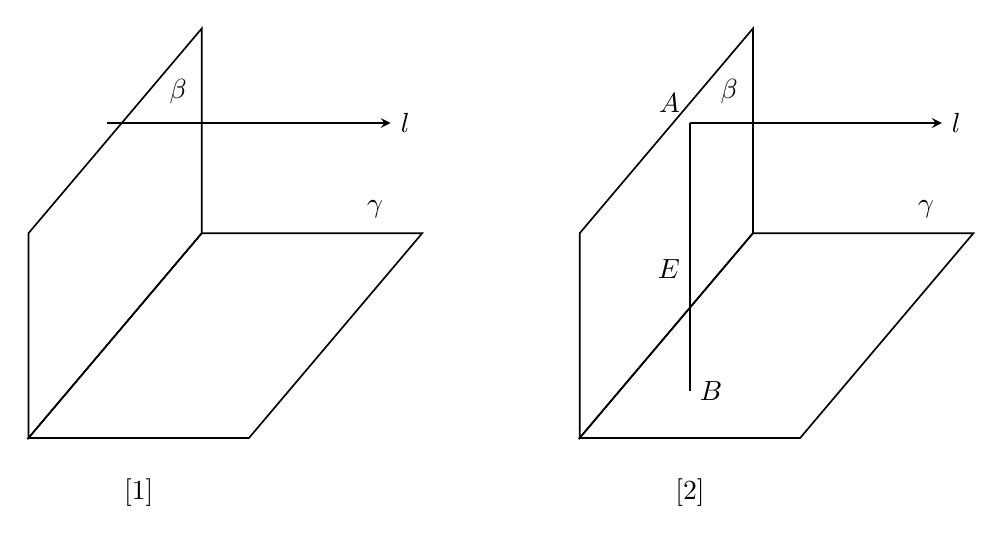
\begin{tikzpicture}[line width=.6pt, >=stealth, font=\normalsize]
  % ---- panel 1 (left) ----
  \begin{scope}[shift={(0,0)}]
    % plane beta (vertical)
    \draw (0,0) -- (2.2,2.6) -- (2.2,5.2) -- (0,2.6) -- cycle;
    % plane gamma (horizontal)
    \draw (0,0) -- (2.2,2.6) -- (5.0,2.6) -- (2.8,0) -- cycle;
    \node at (1.9,4.4) {$\beta$};
    \node at (4.4,2.9) {$\gamma$};
    % line l piercing beta, horizontal
    \draw[->] (1.0,4.0) -- (4.6,4.0) node[right] {$l$};
    \node at (1.4,-0.7) {\bitmapinsertcaption[1]};
  \end{scope}
  % ---- panel 2 (right) ----
  \begin{scope}[shift={(7,0)}]
    % plane beta (vertical)
    \draw (0,0) -- (2.2,2.6) -- (2.2,5.2) -- (0,2.6) -- cycle;
    % plane gamma (horizontal)
    \draw (0,0) -- (2.2,2.6) -- (5.0,2.6) -- (2.8,0) -- cycle;
    \node at (1.9,4.4) {$\beta$};
    \node at (4.4,2.9) {$\gamma$};
    % intersection m is the shared edge from corner
    % line l horizontal from A
    \coordinate (A2) at (1.4,4.0);
    \draw[->] (A2) -- (4.6,4.0) node[right] {$l$};
    % segment AB vertical, crossing m at E
    \coordinate (B2) at (1.4,0.6);
    \coordinate (E2) at (1.4,2.15);
    \node[above left] at (A2) {$A$};
    \draw (A2) -- (B2);
    \node[right] at (B2) {$B$};
    \node[left] at (E2) {$E$};
    \node at (1.4,-0.7) {\bitmapinsertcaption[2]};
  \end{scope}
\end{tikzpicture}
